% Options for packages loaded elsewhere
\PassOptionsToPackage{unicode}{hyperref}
\PassOptionsToPackage{hyphens}{url}
%
\documentclass[
]{article}
\usepackage{amsmath,amssymb}
\usepackage{iftex}
\ifPDFTeX
  \usepackage[T1]{fontenc}
  \usepackage[utf8]{inputenc}
  \usepackage{textcomp} % provide euro and other symbols
\else % if luatex or xetex
  \usepackage{unicode-math} % this also loads fontspec
  \defaultfontfeatures{Scale=MatchLowercase}
  \defaultfontfeatures[\rmfamily]{Ligatures=TeX,Scale=1}
\fi
\usepackage{lmodern}
\ifPDFTeX\else
  % xetex/luatex font selection
\fi
% Use upquote if available, for straight quotes in verbatim environments
\IfFileExists{upquote.sty}{\usepackage{upquote}}{}
\IfFileExists{microtype.sty}{% use microtype if available
  \usepackage[]{microtype}
  \UseMicrotypeSet[protrusion]{basicmath} % disable protrusion for tt fonts
}{}
\makeatletter
\@ifundefined{KOMAClassName}{% if non-KOMA class
  \IfFileExists{parskip.sty}{%
    \usepackage{parskip}
  }{% else
    \setlength{\parindent}{0pt}
    \setlength{\parskip}{6pt plus 2pt minus 1pt}}
}{% if KOMA class
  \KOMAoptions{parskip=half}}
\makeatother
\usepackage{xcolor}
\usepackage[margin=1in]{geometry}
\usepackage{color}
\usepackage{fancyvrb}
\newcommand{\VerbBar}{|}
\newcommand{\VERB}{\Verb[commandchars=\\\{\}]}
\DefineVerbatimEnvironment{Highlighting}{Verbatim}{commandchars=\\\{\}}
% Add ',fontsize=\small' for more characters per line
\usepackage{framed}
\definecolor{shadecolor}{RGB}{248,248,248}
\newenvironment{Shaded}{\begin{snugshade}}{\end{snugshade}}
\newcommand{\AlertTok}[1]{\textcolor[rgb]{0.94,0.16,0.16}{#1}}
\newcommand{\AnnotationTok}[1]{\textcolor[rgb]{0.56,0.35,0.01}{\textbf{\textit{#1}}}}
\newcommand{\AttributeTok}[1]{\textcolor[rgb]{0.13,0.29,0.53}{#1}}
\newcommand{\BaseNTok}[1]{\textcolor[rgb]{0.00,0.00,0.81}{#1}}
\newcommand{\BuiltInTok}[1]{#1}
\newcommand{\CharTok}[1]{\textcolor[rgb]{0.31,0.60,0.02}{#1}}
\newcommand{\CommentTok}[1]{\textcolor[rgb]{0.56,0.35,0.01}{\textit{#1}}}
\newcommand{\CommentVarTok}[1]{\textcolor[rgb]{0.56,0.35,0.01}{\textbf{\textit{#1}}}}
\newcommand{\ConstantTok}[1]{\textcolor[rgb]{0.56,0.35,0.01}{#1}}
\newcommand{\ControlFlowTok}[1]{\textcolor[rgb]{0.13,0.29,0.53}{\textbf{#1}}}
\newcommand{\DataTypeTok}[1]{\textcolor[rgb]{0.13,0.29,0.53}{#1}}
\newcommand{\DecValTok}[1]{\textcolor[rgb]{0.00,0.00,0.81}{#1}}
\newcommand{\DocumentationTok}[1]{\textcolor[rgb]{0.56,0.35,0.01}{\textbf{\textit{#1}}}}
\newcommand{\ErrorTok}[1]{\textcolor[rgb]{0.64,0.00,0.00}{\textbf{#1}}}
\newcommand{\ExtensionTok}[1]{#1}
\newcommand{\FloatTok}[1]{\textcolor[rgb]{0.00,0.00,0.81}{#1}}
\newcommand{\FunctionTok}[1]{\textcolor[rgb]{0.13,0.29,0.53}{\textbf{#1}}}
\newcommand{\ImportTok}[1]{#1}
\newcommand{\InformationTok}[1]{\textcolor[rgb]{0.56,0.35,0.01}{\textbf{\textit{#1}}}}
\newcommand{\KeywordTok}[1]{\textcolor[rgb]{0.13,0.29,0.53}{\textbf{#1}}}
\newcommand{\NormalTok}[1]{#1}
\newcommand{\OperatorTok}[1]{\textcolor[rgb]{0.81,0.36,0.00}{\textbf{#1}}}
\newcommand{\OtherTok}[1]{\textcolor[rgb]{0.56,0.35,0.01}{#1}}
\newcommand{\PreprocessorTok}[1]{\textcolor[rgb]{0.56,0.35,0.01}{\textit{#1}}}
\newcommand{\RegionMarkerTok}[1]{#1}
\newcommand{\SpecialCharTok}[1]{\textcolor[rgb]{0.81,0.36,0.00}{\textbf{#1}}}
\newcommand{\SpecialStringTok}[1]{\textcolor[rgb]{0.31,0.60,0.02}{#1}}
\newcommand{\StringTok}[1]{\textcolor[rgb]{0.31,0.60,0.02}{#1}}
\newcommand{\VariableTok}[1]{\textcolor[rgb]{0.00,0.00,0.00}{#1}}
\newcommand{\VerbatimStringTok}[1]{\textcolor[rgb]{0.31,0.60,0.02}{#1}}
\newcommand{\WarningTok}[1]{\textcolor[rgb]{0.56,0.35,0.01}{\textbf{\textit{#1}}}}
\usepackage{graphicx}
\makeatletter
\def\maxwidth{\ifdim\Gin@nat@width>\linewidth\linewidth\else\Gin@nat@width\fi}
\def\maxheight{\ifdim\Gin@nat@height>\textheight\textheight\else\Gin@nat@height\fi}
\makeatother
% Scale images if necessary, so that they will not overflow the page
% margins by default, and it is still possible to overwrite the defaults
% using explicit options in \includegraphics[width, height, ...]{}
\setkeys{Gin}{width=\maxwidth,height=\maxheight,keepaspectratio}
% Set default figure placement to htbp
\makeatletter
\def\fps@figure{htbp}
\makeatother
\setlength{\emergencystretch}{3em} % prevent overfull lines
\providecommand{\tightlist}{%
  \setlength{\itemsep}{0pt}\setlength{\parskip}{0pt}}
\setcounter{secnumdepth}{-\maxdimen} % remove section numbering
\ifLuaTeX
  \usepackage{selnolig}  % disable illegal ligatures
\fi
\IfFileExists{bookmark.sty}{\usepackage{bookmark}}{\usepackage{hyperref}}
\IfFileExists{xurl.sty}{\usepackage{xurl}}{} % add URL line breaks if available
\urlstyle{same}
\hypersetup{
  pdftitle={moodVariability},
  pdfauthor={Ryan Yan},
  hidelinks,
  pdfcreator={LaTeX via pandoc}}

\title{moodVariability}
\author{Ryan Yan}
\date{2024-01-16}

\begin{document}
\maketitle

Paper 1: Specific components of task based mood variability are
associated with specific components of real world mood variability. The
diurnal stuff could go in this paper.

The logic of this paper would be: mood variability is clinically
interesting but difficult and time consuming to measure. You can split
it up into different components but would be nice to assess whether we
can study these components experimentally in the lab. We looked at
whether we could do that by getting people to complete a task, and then
following them up after. We found this specificity in terms of type of
mood variability.

In addition we wondered about diurnal effects in the real world data,
which were associated with noise, not volatility (the missing thing here
would be an analysis of the link between the task and the diurnal
stuff---might not work as diurnal effect is valence specific though).

\hypertarget{library}{%
\section{library}\label{library}}

\begin{Shaded}
\begin{Highlighting}[]
\FunctionTok{source}\NormalTok{(here}\SpecialCharTok{::}\FunctionTok{here}\NormalTok{(}\StringTok{"load\_library.R"}\NormalTok{))}
\end{Highlighting}
\end{Shaded}

\begin{Shaded}
\begin{Highlighting}[]
\FunctionTok{theme\_set}\NormalTok{(}\FunctionTok{theme\_classic}\NormalTok{()}\SpecialCharTok{+}
          \FunctionTok{theme}\NormalTok{(}\AttributeTok{text =} \FunctionTok{element\_text}\NormalTok{(}\AttributeTok{family =} \StringTok{"Helvetica"}\NormalTok{, }\AttributeTok{size =} \DecValTok{10}\NormalTok{)))}
\NormalTok{vmuColor }\OtherTok{\textless{}{-}} \StringTok{"red"}
\NormalTok{noiseColor }\OtherTok{\textless{}{-}} \StringTok{\textquotesingle{}royalblue3\textquotesingle{}}
\NormalTok{muColor }\OtherTok{\textless{}{-}} \StringTok{\textquotesingle{}forestgreen\textquotesingle{}}
\end{Highlighting}
\end{Shaded}

\hypertarget{load-and-combine-data}{%
\section{load and combine data}\label{load-and-combine-data}}

\begin{Shaded}
\begin{Highlighting}[]
\NormalTok{rmarkdown}\SpecialCharTok{::}\FunctionTok{render}\NormalTok{(}\StringTok{"read\_data.Rmd"}\NormalTok{)}
\end{Highlighting}
\end{Shaded}

\begin{verbatim}
##   |                               |                       |   0%  |                               |.                      |   6%                                                 |                               |...                    |  11% [load data]                                     |                               |....                   |  17%                                                 |                               |.....                  |  22% [sort obs. and delete duplicates]               |                               |......                 |  28%                                                 |                               |........               |  33% [calc and aggregate baseline questionnaires]    |                               |.........              |  39%                                                 |                               |..........             |  44% [unnamed-chunk-13]                              |                               |............           |  50%                                                 |                               |.............          |  56% [impoart WoF and make data frame WoF~moodrate]  |                               |..............         |  61%                                                 |                               |...............        |  67% [unnamed-chunk-14]                              |                               |.................      |  72%                                                 |                               |..................     |  78% [read .csv]                                     |                               |...................    |  83%                                                 |                               |....................   |  89% [unnamed-chunk-15]                              |                               |...................... |  94%                                                 |                               |.......................| 100% [unnamed-chunk-16]                                                                                                                                                                     
## /Applications/RStudio.app/Contents/Resources/app/quarto/bin/tools/pandoc +RTS -K512m -RTS read_data.knit.md --to html4 --from markdown+autolink_bare_uris+tex_math_single_backslash --output read_data.html --lua-filter /Library/Frameworks/R.framework/Versions/4.0/Resources/library/rmarkdown/rmarkdown/lua/pagebreak.lua --lua-filter /Library/Frameworks/R.framework/Versions/4.0/Resources/library/rmarkdown/rmarkdown/lua/latex-div.lua --embed-resources --standalone --variable bs3=TRUE --section-divs --template /Library/Frameworks/R.framework/Versions/4.0/Resources/library/rmarkdown/rmd/h/default.html --no-highlight --variable highlightjs=1 --variable theme=bootstrap --mathjax --variable 'mathjax-url=https://mathjax.rstudio.com/latest/MathJax.js?config=TeX-AMS-MML_HTMLorMML' --include-in-header /var/folders/48/c4z661n561sdsq0k31vt8ly80000gn/T//RtmpJGi0GH/rmarkdown-stracdb5e78e4be.html
\end{verbatim}

\hypertarget{part-1-linking-task-and-ema-mood-variability}{%
\section{part 1: Linking task and EMA mood
variability}\label{part-1-linking-task-and-ema-mood-variability}}

\hypertarget{simulation-demonstrating-the-plausibility-of-inferring-long-term-affective-variability-from-task-variability}{%
\subsection{1.1 simulation demonstrating the plausibility of inferring
long-term affective variability from task
variability}\label{simulation-demonstrating-the-plausibility-of-inferring-long-term-affective-variability-from-task-variability}}

\[Affect = setpoint + \sum_{t=1}^{T}event_t(a*e^{b(t-T)})\]

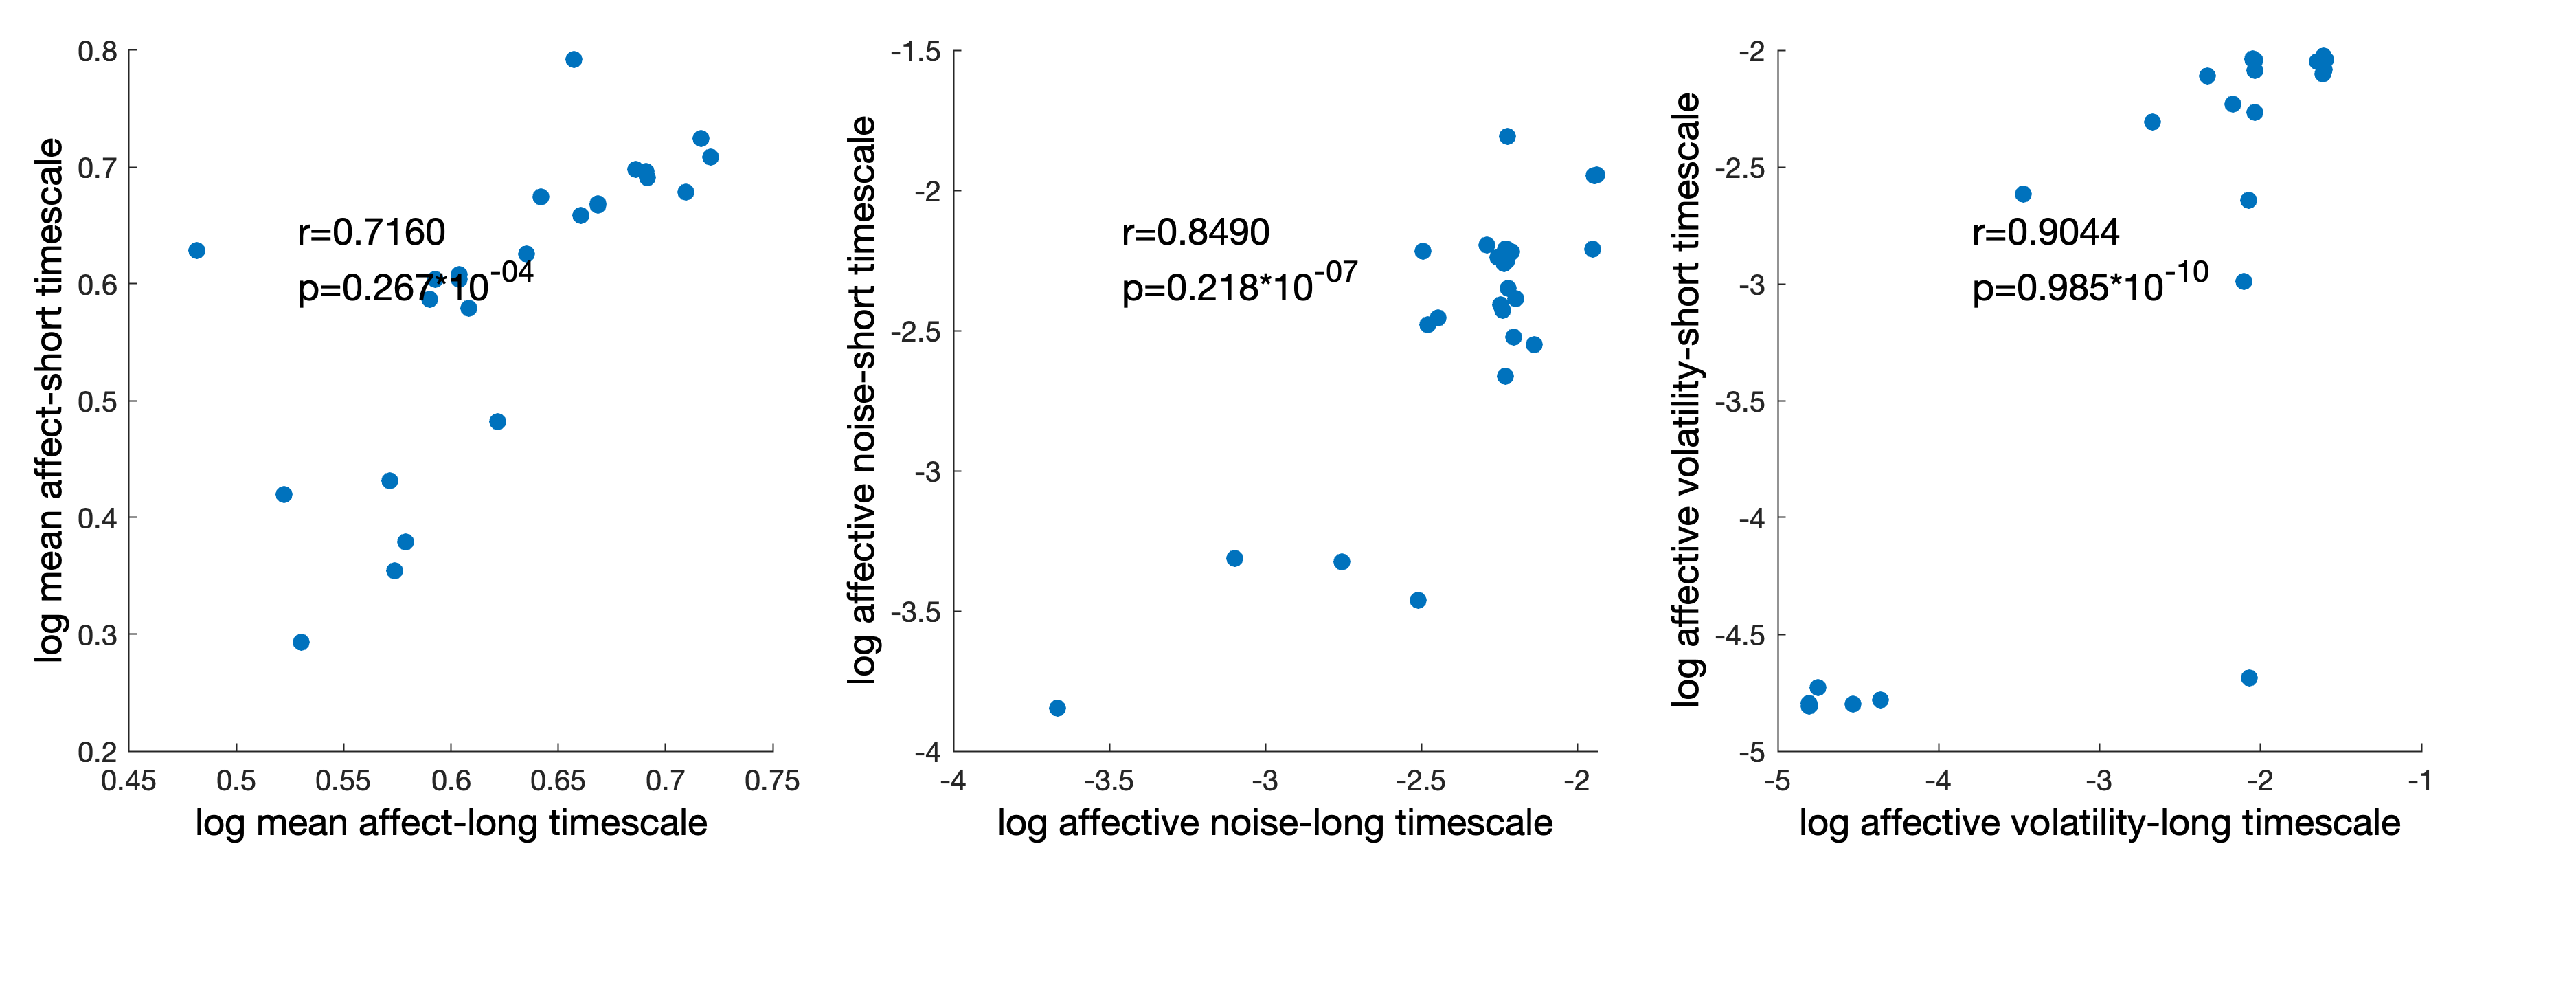
\includegraphics{./figures/figure_SimCorr.png} Figure 1 shows that
affective parameters acquired from a small portion (3\%) of affective
time-series, generally appear to correlate with equivalent parameters
acquired from the full time-series.

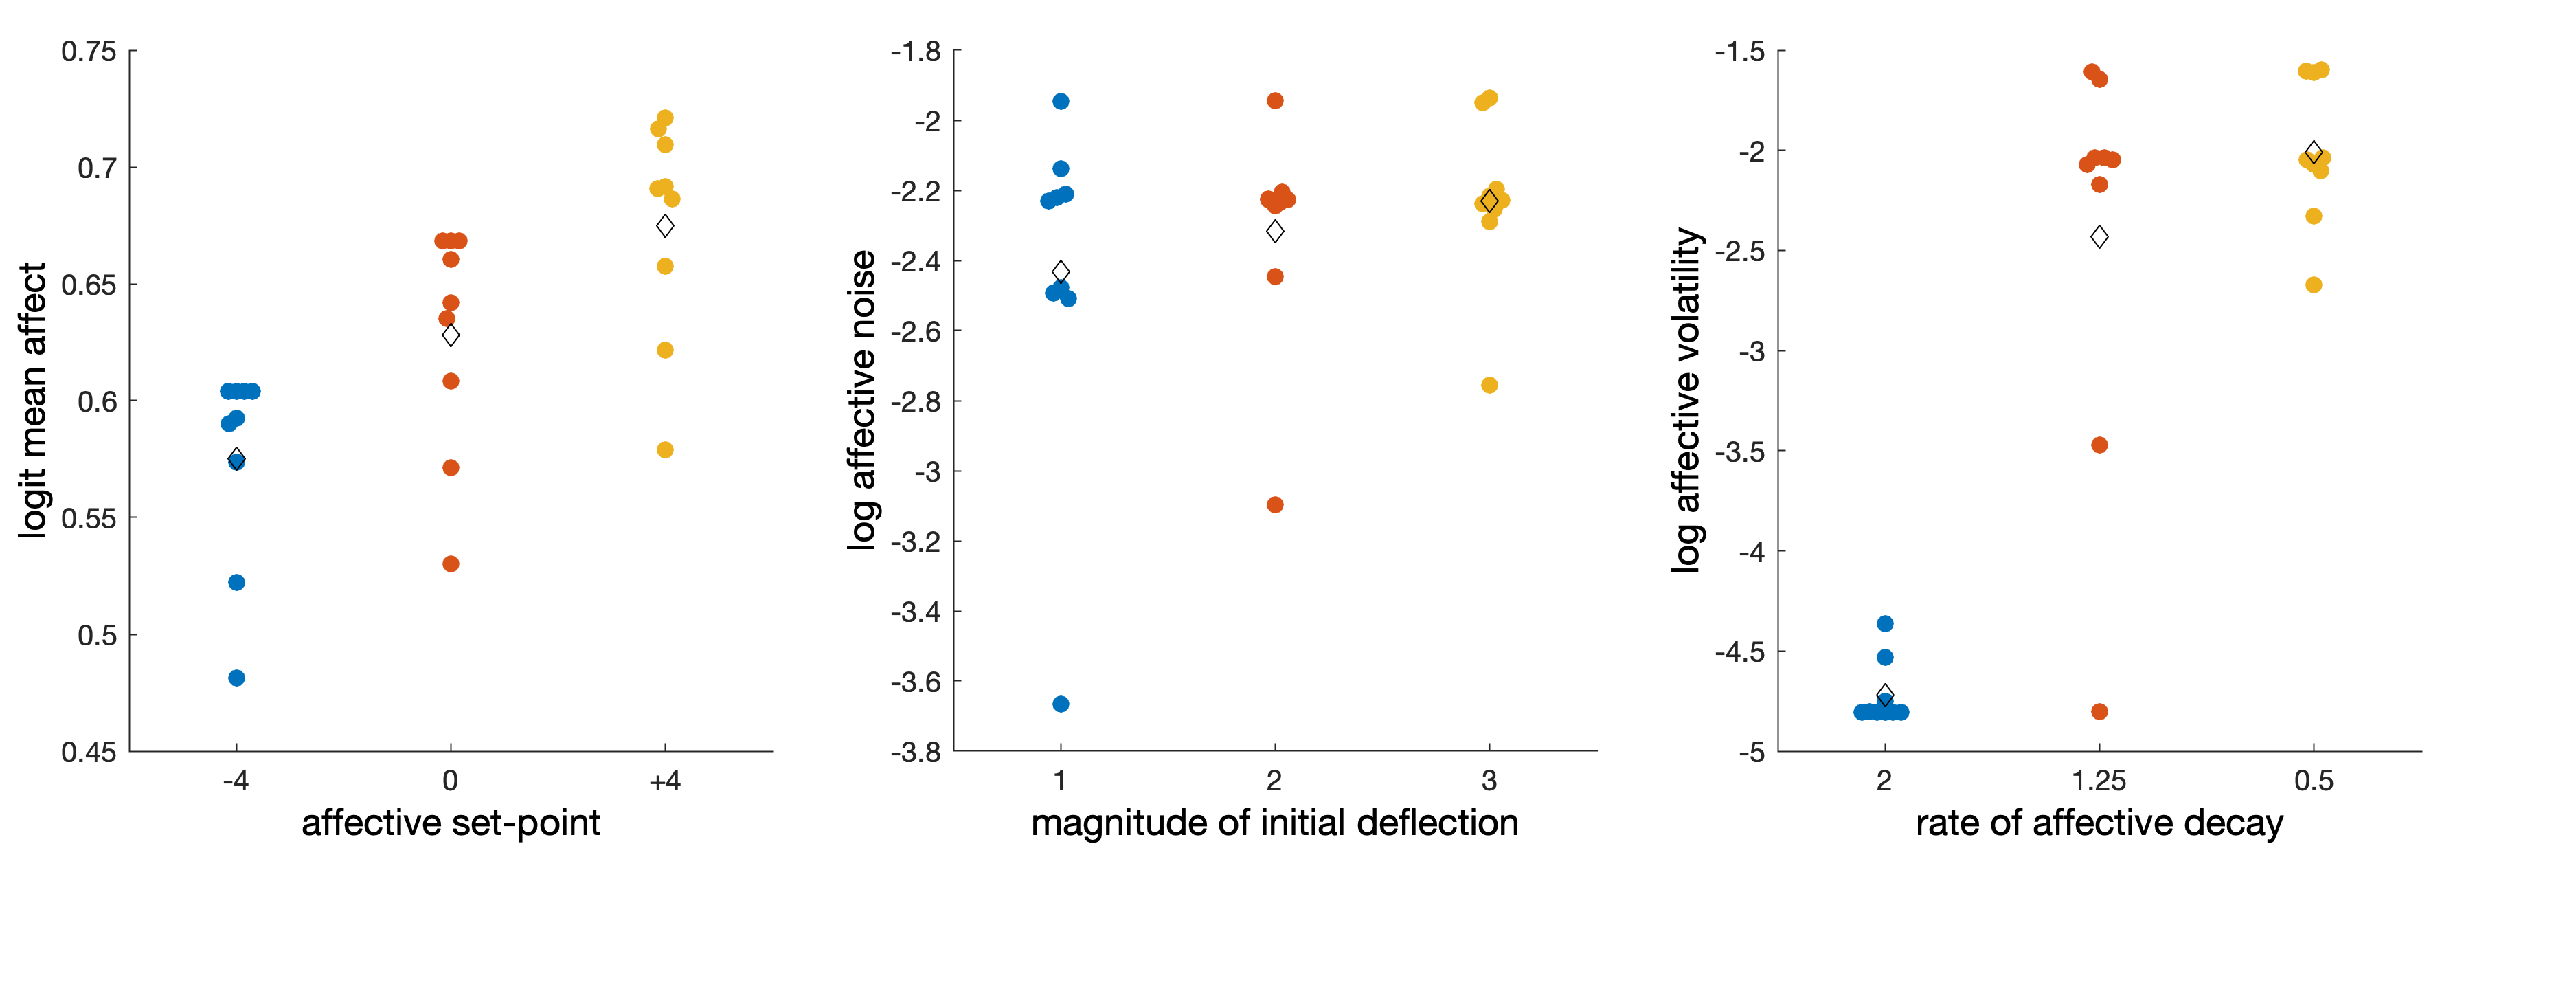
\includegraphics{./figures/figure_SimExpVsbayes.png} As illustrated in
the 3 panels above, the filter's estimated \emph{mu} appears to
generally increase as the affective set point increases, the filter's
estimated \emph{SD} appears to generally increase as the initial
deflection increases and the filter's estimated \emph{vmu} appears to
generally increase as the decay rate decreases.

\hypertarget{dependency-of-gorilla-task-parameters-on-emotional-reactivity}{%
\subsection{1.2 dependency of gorilla task parameters on emotional
reactivity}\label{dependency-of-gorilla-task-parameters-on-emotional-reactivity}}

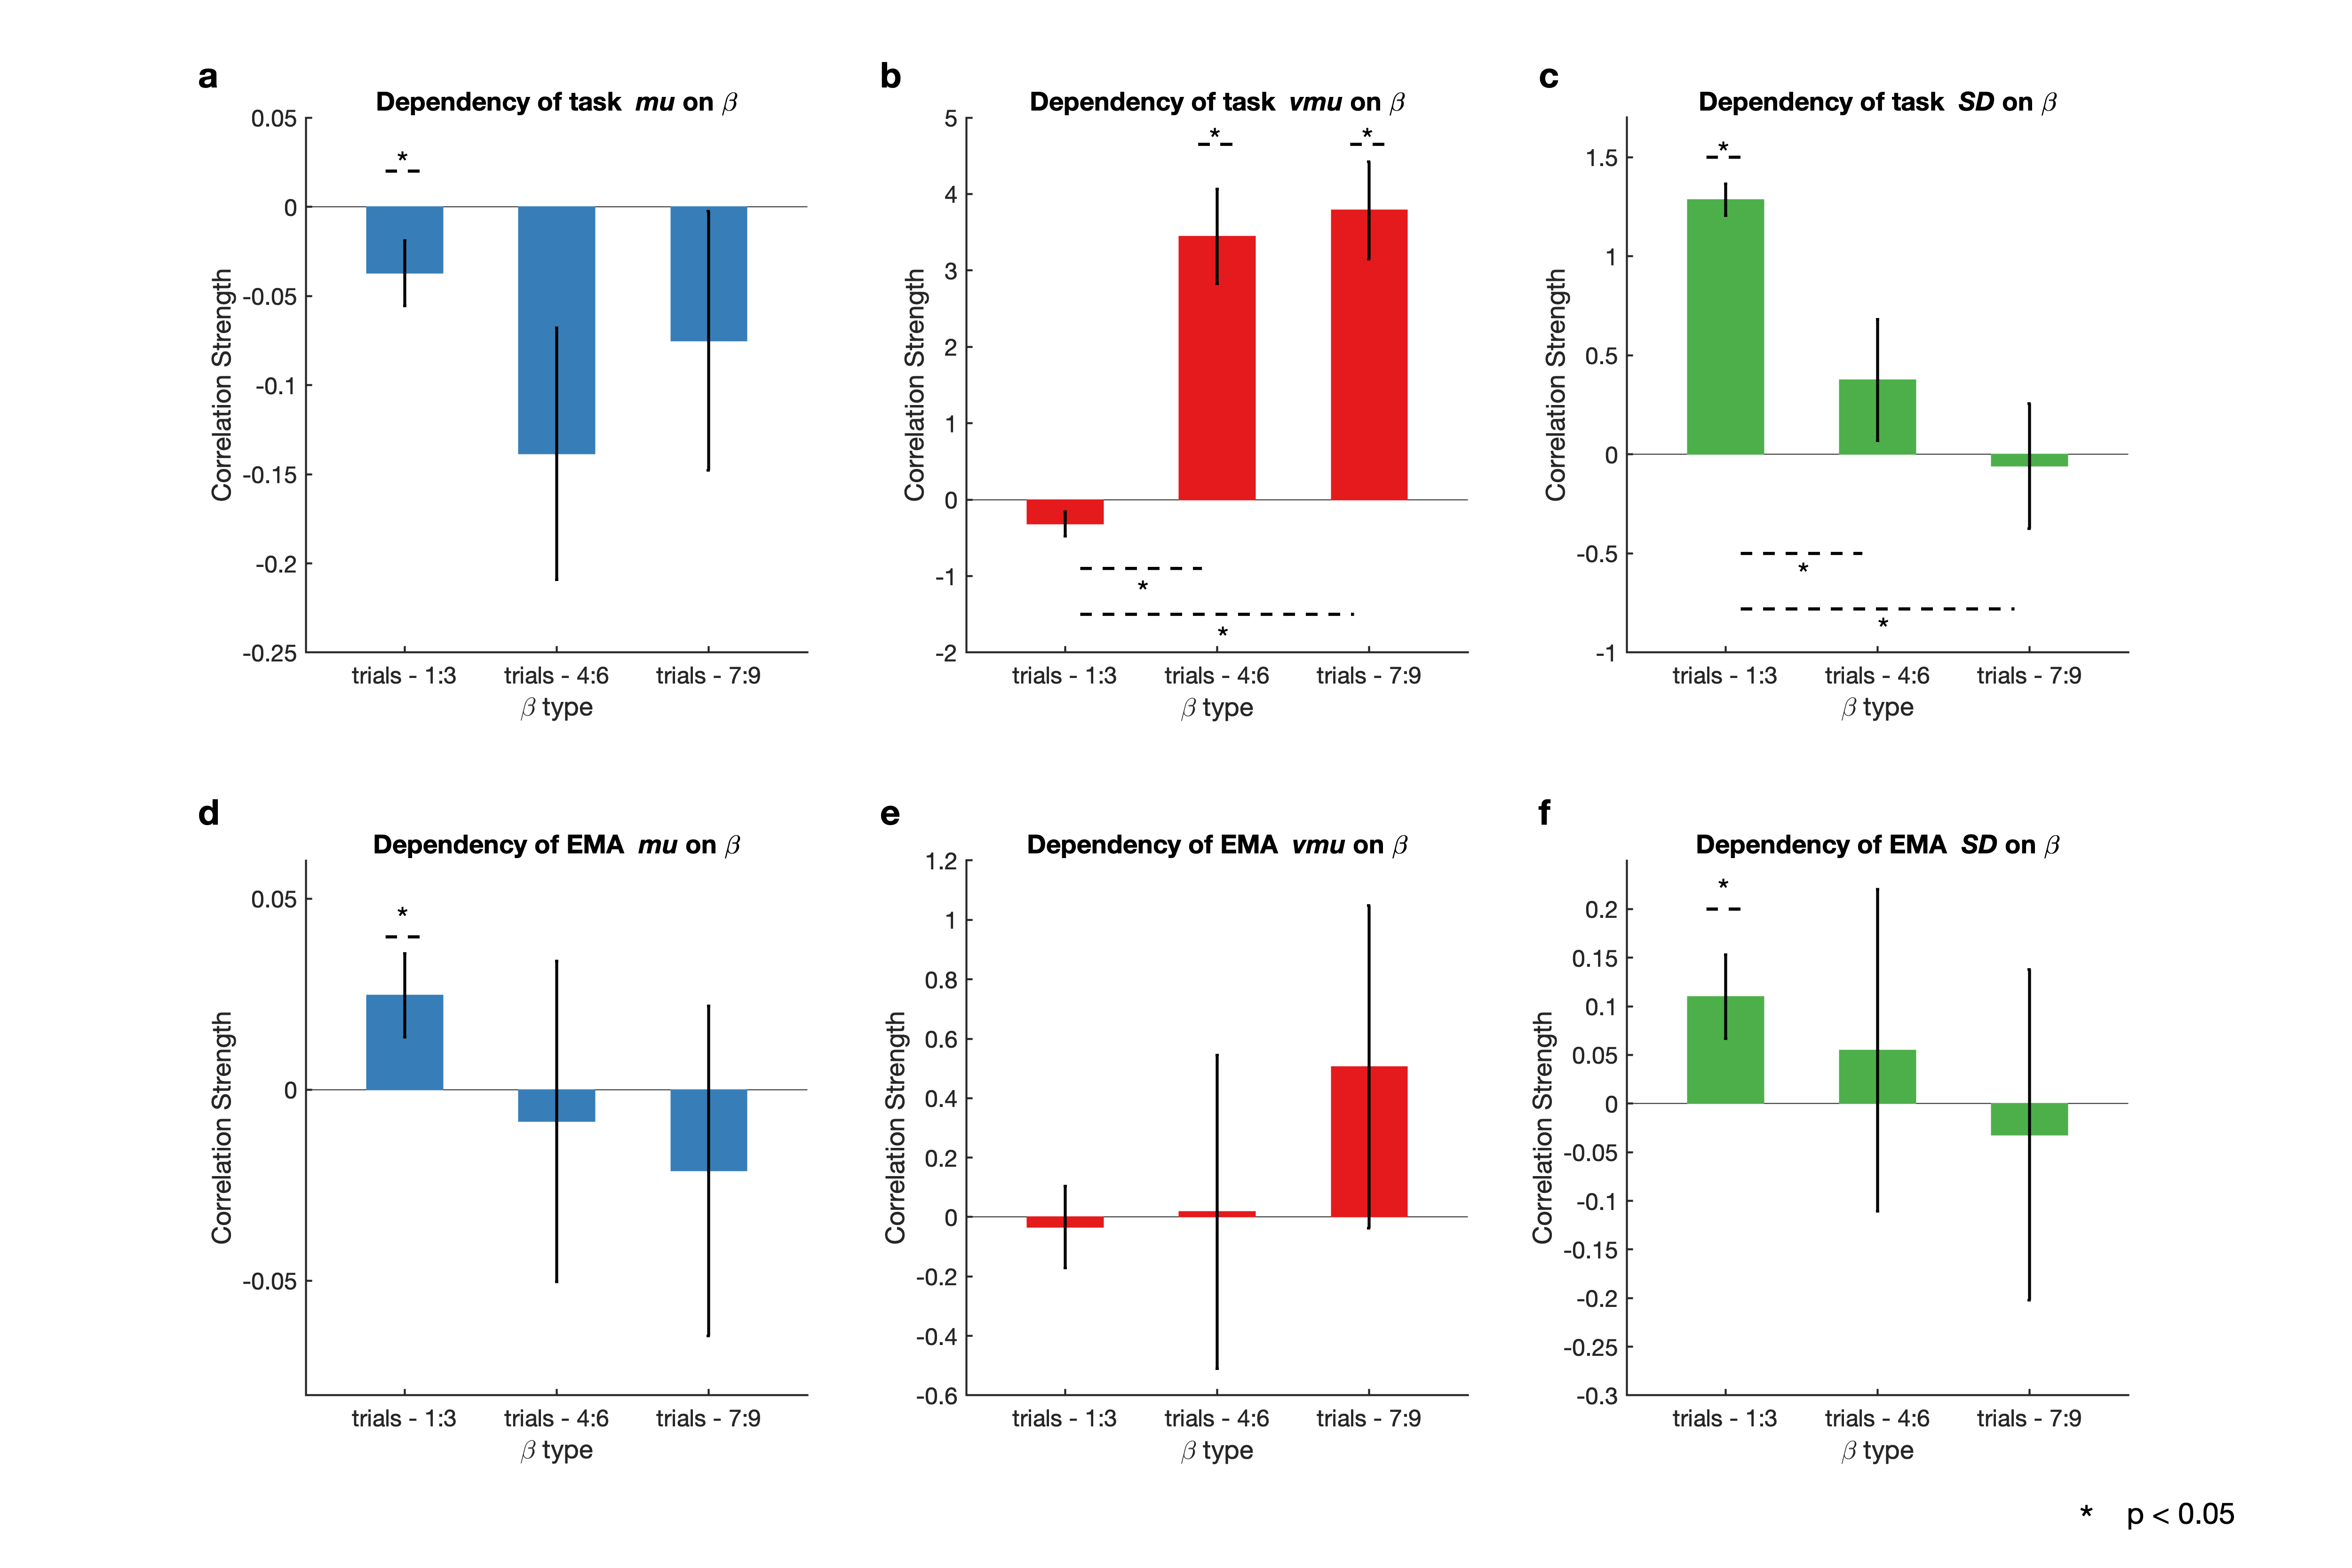
\includegraphics{./figures/figure_Bayes_vs_Betas.png} (a-c) Task
\emph{SD} is associated with the immediate impact of task events, which
is consistent with the idea that it reflects the magnitude of initial
affective deflection from baseline. Task \emph{vmu} is associated with
the persistent impact of task events, which is consistent with the idea
that it reflects the rate at which affect returns to baseline.
Unexpectedly, task \emph{mu} is negatively associated with the immediate
impact of task events, it is unclear what this signifies. (d-f) As with
task \emph{SD}, ESM \emph{SD} is associated with the immediate impact of
task events, which is consistent with the idea that 𝑆𝐷 in everyday life
reflects the magnitude of initial affective deflections from baseline.
ESM \emph{vmu} does not bear any significant relationship to the
duration of responses to task events. ESM \emph{mu} shows the same
pattern of associations as ESM \emph{SD}.

\hypertarget{dependency-of-ema-params-on-task-params}{%
\subsection{1.3 dependency of EMA params on task
params}\label{dependency-of-ema-params-on-task-params}}

\begin{Shaded}
\begin{Highlighting}[]
\FunctionTok{ggplot}\NormalTok{(df\_master, }\FunctionTok{aes}\NormalTok{(}\AttributeTok{x =}\NormalTok{ mean5\_vmu, }\AttributeTok{y =}\NormalTok{ mean5\_vmu\_posminusneg))}\SpecialCharTok{+}
  \FunctionTok{geom\_point}\NormalTok{(}\AttributeTok{size =} \FloatTok{0.5}\NormalTok{)}\SpecialCharTok{+}
  \FunctionTok{geom\_smooth}\NormalTok{(}\AttributeTok{method =} \StringTok{"lm"}\NormalTok{, }\AttributeTok{color =}\NormalTok{ vmuColor, }\AttributeTok{fill =}\NormalTok{ vmuColor) }\SpecialCharTok{+}
  \FunctionTok{stat\_poly\_eq}\NormalTok{(}\FunctionTok{use\_label}\NormalTok{(}\FunctionTok{c}\NormalTok{(}\StringTok{"R2"}\NormalTok{,}\StringTok{"p"}\NormalTok{)))}\SpecialCharTok{+}
  \FunctionTok{labs}\NormalTok{(}\AttributeTok{title =}\StringTok{"dependency of task parames on EMA params"}\NormalTok{,}
       \AttributeTok{x =} \StringTok{"task volatility"}\NormalTok{,}
       \AttributeTok{y =} \StringTok{"EMA volatility"}\NormalTok{)}\SpecialCharTok{+}
\FunctionTok{ggplot}\NormalTok{(df\_master, }\FunctionTok{aes}\NormalTok{(}\AttributeTok{x =}\NormalTok{ mean\_mu, }\AttributeTok{y =}\NormalTok{ mean\_mu\_posminusneg))}\SpecialCharTok{+}
  \FunctionTok{geom\_point}\NormalTok{(}\AttributeTok{size =} \FloatTok{0.5}\NormalTok{)}\SpecialCharTok{+}
  \FunctionTok{geom\_smooth}\NormalTok{(}\AttributeTok{method =} \StringTok{"lm"}\NormalTok{, }\AttributeTok{color =}\NormalTok{ muColor, }\AttributeTok{fill =}\NormalTok{ muColor) }\SpecialCharTok{+}
  \FunctionTok{stat\_poly\_eq}\NormalTok{(}\FunctionTok{use\_label}\NormalTok{(}\FunctionTok{c}\NormalTok{(}\StringTok{"R2"}\NormalTok{,}\StringTok{"p"}\NormalTok{)))}\SpecialCharTok{+}
  \FunctionTok{labs}\NormalTok{(}\AttributeTok{x =} \StringTok{"task mean"}\NormalTok{,}
       \AttributeTok{y =} \StringTok{"EMA mean"}\NormalTok{)}\SpecialCharTok{+}
\FunctionTok{ggplot}\NormalTok{(df\_master, }\FunctionTok{aes}\NormalTok{(}\AttributeTok{x =}\NormalTok{ mean\_s, }\AttributeTok{y =}\NormalTok{ mean\_s\_posminusneg))}\SpecialCharTok{+}
  \FunctionTok{geom\_point}\NormalTok{(}\AttributeTok{size =} \FloatTok{0.5}\NormalTok{)}\SpecialCharTok{+}
  \FunctionTok{geom\_smooth}\NormalTok{(}\AttributeTok{method =} \StringTok{"lm"}\NormalTok{, }\AttributeTok{color =}\NormalTok{ noiseColor, }\AttributeTok{fill =}\NormalTok{ noiseColor) }\SpecialCharTok{+}
  \FunctionTok{stat\_poly\_eq}\NormalTok{(}\FunctionTok{use\_label}\NormalTok{(}\FunctionTok{c}\NormalTok{(}\StringTok{"R2"}\NormalTok{,}\StringTok{"p"}\NormalTok{)))}\SpecialCharTok{+}
  \FunctionTok{labs}\NormalTok{(}\AttributeTok{x =} \StringTok{"task noise"}\NormalTok{,}
       \AttributeTok{y =} \StringTok{"EMA noise"}\NormalTok{)}
\end{Highlighting}
\end{Shaded}

\begin{verbatim}
## `geom_smooth()` using formula = 'y ~ x'
## `geom_smooth()` using formula = 'y ~ x'
## `geom_smooth()` using formula = 'y ~ x'
\end{verbatim}

\includegraphics{moodVariability_task_files/figure-latex/unnamed-chunk-4-1.pdf}

\begin{Shaded}
\begin{Highlighting}[]
\FunctionTok{summary}\NormalTok{(}\FunctionTok{lm}\NormalTok{(mean5\_vmu }\SpecialCharTok{\textasciitilde{}}\NormalTok{ mean5\_vmu\_posminusneg }\SpecialCharTok{+}\NormalTok{ mean\_mu }\SpecialCharTok{+}\NormalTok{ mean\_s, df\_master))}
\end{Highlighting}
\end{Shaded}

\begin{verbatim}
## 
## Call:
## lm(formula = mean5_vmu ~ mean5_vmu_posminusneg + mean_mu + mean_s, 
##     data = df_master)
## 
## Residuals:
##     Min      1Q  Median      3Q     Max 
## -2.3476 -0.6786 -0.1164  0.7741  2.5660 
## 
## Coefficients:
##                       Estimate Std. Error t value Pr(>|t|)    
## (Intercept)           -1.21944    0.36721  -3.321 0.000996 ***
## mean5_vmu_posminusneg  0.11683    0.05064   2.307 0.021668 *  
## mean_mu               -2.00947    0.55900  -3.595 0.000374 ***
## mean_s                 0.30138    0.08507   3.543 0.000452 ***
## ---
## Signif. codes:  0 '***' 0.001 '**' 0.01 '*' 0.05 '.' 0.1 ' ' 1
## 
## Residual standard error: 0.9337 on 335 degrees of freedom
## Multiple R-squared:  0.09627,    Adjusted R-squared:  0.08817 
## F-statistic:  11.9 on 3 and 335 DF,  p-value: 2.021e-07
\end{verbatim}

\begin{Shaded}
\begin{Highlighting}[]
\FunctionTok{summary}\NormalTok{(}\FunctionTok{lm}\NormalTok{(mean\_mu }\SpecialCharTok{\textasciitilde{}}\NormalTok{ mean\_mu\_posminusneg }\SpecialCharTok{+}\NormalTok{ mean5\_vmu }\SpecialCharTok{+}\NormalTok{ mean\_s, df\_master))}
\end{Highlighting}
\end{Shaded}

\begin{verbatim}
## 
## Call:
## lm(formula = mean_mu ~ mean_mu_posminusneg + mean5_vmu + mean_s, 
##     data = df_master)
## 
## Residuals:
##      Min       1Q   Median       3Q      Max 
## -0.40424 -0.05378 -0.00399  0.05241  0.18780 
## 
## Coefficients:
##                      Estimate Std. Error t value Pr(>|t|)    
## (Intercept)          0.225320   0.039657   5.682 2.90e-08 ***
## mean_mu_posminusneg  0.422104   0.056450   7.477 6.69e-13 ***
## mean5_vmu           -0.018353   0.004720  -3.888 0.000122 ***
## mean_s              -0.026348   0.007689  -3.427 0.000687 ***
## ---
## Signif. codes:  0 '***' 0.001 '**' 0.01 '*' 0.05 '.' 0.1 ' ' 1
## 
## Residual standard error: 0.08291 on 335 degrees of freedom
## Multiple R-squared:  0.1981, Adjusted R-squared:  0.1909 
## F-statistic: 27.59 on 3 and 335 DF,  p-value: 5.743e-16
\end{verbatim}

\begin{Shaded}
\begin{Highlighting}[]
\FunctionTok{summary}\NormalTok{(}\FunctionTok{lm}\NormalTok{(mean\_s }\SpecialCharTok{\textasciitilde{}}\NormalTok{ mean\_s\_posminusneg }\SpecialCharTok{+}\NormalTok{ mean\_mu }\SpecialCharTok{+}\NormalTok{ mean5\_vmu, df\_master))}
\end{Highlighting}
\end{Shaded}

\begin{verbatim}
## 
## Call:
## lm(formula = mean_s ~ mean_s_posminusneg + mean_mu + mean5_vmu, 
##     data = df_master)
## 
## Residuals:
##      Min       1Q   Median       3Q      Max 
## -1.93995 -0.31097  0.00134  0.38396  1.35799 
## 
## Coefficients:
##                    Estimate Std. Error t value Pr(>|t|)    
## (Intercept)        -0.14617    0.24739  -0.591 0.555033    
## mean_s_posminusneg  0.36112    0.09917   3.642 0.000314 ***
## mean_mu            -0.70626    0.35157  -2.009 0.045350 *  
## mean5_vmu           0.10412    0.03317   3.139 0.001848 ** 
## ---
## Signif. codes:  0 '***' 0.001 '**' 0.01 '*' 0.05 '.' 0.1 ' ' 1
## 
## Residual standard error: 0.579 on 335 degrees of freedom
## Multiple R-squared:  0.09509,    Adjusted R-squared:  0.08698 
## F-statistic: 11.73 on 3 and 335 DF,  p-value: 2.5e-07
\end{verbatim}

\begin{Shaded}
\begin{Highlighting}[]
\FunctionTok{chart.Correlation}\NormalTok{(df\_master }\SpecialCharTok{\%\textgreater{}\%} 
\NormalTok{                    dplyr}\SpecialCharTok{::}\FunctionTok{select}\NormalTok{(mean5\_vmu\_posminusneg,mean\_s\_posminusneg,mean\_mu\_posminusneg, }
\NormalTok{                                 mean5\_vmu,mean\_mu,mean\_s) }\SpecialCharTok{\%\textgreater{}\%} 
                    \FunctionTok{rename}\NormalTok{(}\AttributeTok{task\_vmu =}\NormalTok{ mean5\_vmu,}
                           \AttributeTok{task\_sd =}\NormalTok{ mean\_s,}
                           \AttributeTok{task\_mu =}\NormalTok{ mean\_mu,}
                           \AttributeTok{ema\_vmu =}\NormalTok{ mean5\_vmu\_posminusneg,}
                           \AttributeTok{ema\_sd =}\NormalTok{ mean\_s\_posminusneg,}
                           \AttributeTok{ema\_mu =}\NormalTok{ mean\_mu\_posminusneg))}
\end{Highlighting}
\end{Shaded}

\includegraphics{moodVariability_task_files/figure-latex/unnamed-chunk-5-1.pdf}

Task affect variables are specifically associated with their ESM
counterparts when controlling for other task variables. The only
exception is ESM \emph{mu} which was additionally associated with task
\emph{SD}.

\hypertarget{part-2-relationship-between-ema-and-baseline-questionnaires}{%
\section{part 2: Relationship between EMA and baseline
questionnaires}\label{part-2-relationship-between-ema-and-baseline-questionnaires}}

\hypertarget{ema-summary-statistics-and-baseline-questionnaires-gist-poor-differentiation-between-mean-and-se}{%
\subsection{2.1 EMA summary statistics and baseline questionnaires
(gist: poor differentiation between mean and
se)}\label{ema-summary-statistics-and-baseline-questionnaires-gist-poor-differentiation-between-mean-and-se}}

P.S. We used PA minus NA because it's most comparative with the analog
scale
\includegraphics{moodVariability_task_files/figure-latex/unnamed-chunk-6-1.pdf}

\hypertarget{ema-bayes-params-and-baseline-questionnaires}{%
\subsection{2.2 EMA bayes params and baseline
questionnaires}\label{ema-bayes-params-and-baseline-questionnaires}}

\emph{Ask Mike here: how to justify using posminusneg vs.~pos and neg
separately?}

\hypertarget{when-using-the-difference-score-pa-minus-na-we-see-that-the-noise-of-this-net-mood-rating-is-correlated-with-hps-mu-is-correlated-with-teps-and-negative-affectivity-in-the-expected-direction.}{%
\subsubsection{When using the difference score (PA minus NA), we see
that the noise of this `net mood rating' is correlated with HPS; mu is
correlated with TEPS and negative affectivity in the expected
direction.}\label{when-using-the-difference-score-pa-minus-na-we-see-that-the-noise-of-this-net-mood-rating-is-correlated-with-hps-mu-is-correlated-with-teps-and-negative-affectivity-in-the-expected-direction.}}

\begin{Shaded}
\begin{Highlighting}[]
\FunctionTok{chart.Correlation}\NormalTok{(df\_master }\SpecialCharTok{\%\textgreater{}\%} 
\NormalTok{                    dplyr}\SpecialCharTok{::}\FunctionTok{select}\NormalTok{(TEPS\_sum,HPS\_sum,CESD\_sum, STAI\_TA\_sum,STAI\_TA\_sum,}
\NormalTok{                           mean5\_vmu\_posminusneg,mean\_mu\_posminusneg,mean\_s\_posminusneg))}
\end{Highlighting}
\end{Shaded}

\includegraphics{moodVariability_task_files/figure-latex/unnamed-chunk-7-1.pdf}

\hypertarget{teps-is-positively-associated-with-task-sd.-however-considering-from-section-1.3-that-task-sd-is-associated-with-ema-mu-we-want-to-control-for-ema-mu.-after-controlling-the-correlation-is-still-significant-at-p-.05.}{%
\subsubsection{TEPS is positively associated with task SD. However,
considering from section 1.3 that task SD is associated with EMA mu, we
want to control for EMA mu. After controlling, the correlation is still
significant at p \textless{}
.05.}\label{teps-is-positively-associated-with-task-sd.-however-considering-from-section-1.3-that-task-sd-is-associated-with-ema-mu-we-want-to-control-for-ema-mu.-after-controlling-the-correlation-is-still-significant-at-p-.05.}}

\begin{Shaded}
\begin{Highlighting}[]
\FunctionTok{ggplot}\NormalTok{(df\_master, }\FunctionTok{aes}\NormalTok{(}\AttributeTok{x =}\NormalTok{ TEPS\_sum, }\AttributeTok{y =}\NormalTok{ mean5\_vmu))}\SpecialCharTok{+}
  \FunctionTok{geom\_point}\NormalTok{(}\AttributeTok{size =} \FloatTok{0.5}\NormalTok{)}\SpecialCharTok{+}
  \FunctionTok{geom\_smooth}\NormalTok{(}\AttributeTok{method =} \StringTok{"lm"}\NormalTok{, }\AttributeTok{fill =} \StringTok{\textquotesingle{}grey\textquotesingle{}}\NormalTok{, }\AttributeTok{color =} \StringTok{\textquotesingle{}grey\textquotesingle{}}\NormalTok{) }\SpecialCharTok{+}
  \FunctionTok{stat\_poly\_eq}\NormalTok{(}\FunctionTok{use\_label}\NormalTok{(}\FunctionTok{c}\NormalTok{(}\StringTok{"R2"}\NormalTok{,}\StringTok{"p"}\NormalTok{)))}\SpecialCharTok{+}
  \FunctionTok{labs}\NormalTok{(}\AttributeTok{y =} \StringTok{"task mood volatility"}\NormalTok{)}\SpecialCharTok{+}
\FunctionTok{ggplot}\NormalTok{(df\_master, }\FunctionTok{aes}\NormalTok{(}\AttributeTok{x =}\NormalTok{ TEPS\_sum, }\AttributeTok{y =}\NormalTok{ mean\_s))}\SpecialCharTok{+}
  \FunctionTok{geom\_point}\NormalTok{(}\AttributeTok{size =} \FloatTok{0.5}\NormalTok{)}\SpecialCharTok{+}
  \FunctionTok{geom\_smooth}\NormalTok{(}\AttributeTok{method =} \StringTok{"lm"}\NormalTok{, }\AttributeTok{color =}\NormalTok{ noiseColor, }\AttributeTok{fill =}\NormalTok{ noiseColor) }\SpecialCharTok{+}
  \FunctionTok{stat\_poly\_eq}\NormalTok{(}\FunctionTok{use\_label}\NormalTok{(}\FunctionTok{c}\NormalTok{(}\StringTok{"R2"}\NormalTok{,}\StringTok{"p"}\NormalTok{)))}\SpecialCharTok{+}
  \FunctionTok{labs}\NormalTok{(}\AttributeTok{y =} \StringTok{"task mood noise"}\NormalTok{)}\SpecialCharTok{+}
\FunctionTok{ggplot}\NormalTok{(df\_master, }\FunctionTok{aes}\NormalTok{(}\AttributeTok{x =}\NormalTok{ HPS\_sum, }\AttributeTok{y =}\NormalTok{ mean5\_vmu))}\SpecialCharTok{+}
  \FunctionTok{geom\_point}\NormalTok{(}\AttributeTok{size =} \FloatTok{0.5}\NormalTok{)}\SpecialCharTok{+}
  \FunctionTok{geom\_smooth}\NormalTok{(}\AttributeTok{method =} \StringTok{"lm"}\NormalTok{, }\AttributeTok{fill =} \StringTok{\textquotesingle{}grey\textquotesingle{}}\NormalTok{, }\AttributeTok{color =} \StringTok{\textquotesingle{}grey\textquotesingle{}}\NormalTok{) }\SpecialCharTok{+}
  \FunctionTok{stat\_poly\_eq}\NormalTok{(}\FunctionTok{use\_label}\NormalTok{(}\FunctionTok{c}\NormalTok{(}\StringTok{"R2"}\NormalTok{,}\StringTok{"p"}\NormalTok{)))}\SpecialCharTok{+}
  \FunctionTok{labs}\NormalTok{(}\AttributeTok{y =} \StringTok{"task mood volatility"}\NormalTok{)}\SpecialCharTok{+}
\FunctionTok{ggplot}\NormalTok{(df\_master, }\FunctionTok{aes}\NormalTok{(}\AttributeTok{x =}\NormalTok{ HPS\_sum, }\AttributeTok{y =}\NormalTok{ mean\_s))}\SpecialCharTok{+}
  \FunctionTok{geom\_point}\NormalTok{(}\AttributeTok{size =} \FloatTok{0.5}\NormalTok{)}\SpecialCharTok{+}
  \FunctionTok{geom\_smooth}\NormalTok{(}\AttributeTok{method =} \StringTok{"lm"}\NormalTok{, }\AttributeTok{fill =} \StringTok{\textquotesingle{}grey\textquotesingle{}}\NormalTok{, }\AttributeTok{color =} \StringTok{\textquotesingle{}grey\textquotesingle{}}\NormalTok{) }\SpecialCharTok{+}
  \FunctionTok{stat\_poly\_eq}\NormalTok{(}\FunctionTok{use\_label}\NormalTok{(}\FunctionTok{c}\NormalTok{(}\StringTok{"R2"}\NormalTok{,}\StringTok{"p"}\NormalTok{))) }\SpecialCharTok{+}
  \FunctionTok{plot\_layout}\NormalTok{(}\AttributeTok{nrow =} \DecValTok{1}\NormalTok{)}
\end{Highlighting}
\end{Shaded}

\begin{verbatim}
## `geom_smooth()` using formula = 'y ~ x'
## `geom_smooth()` using formula = 'y ~ x'
## `geom_smooth()` using formula = 'y ~ x'
## `geom_smooth()` using formula = 'y ~ x'
\end{verbatim}

\includegraphics{moodVariability_task_files/figure-latex/unnamed-chunk-8-1.pdf}

\begin{Shaded}
\begin{Highlighting}[]
  \FunctionTok{labs}\NormalTok{(}\AttributeTok{y =} \StringTok{"task mood noise"}\NormalTok{)}
\end{Highlighting}
\end{Shaded}

\begin{verbatim}
## $y
## [1] "task mood noise"
## 
## attr(,"class")
## [1] "labels"
\end{verbatim}

\begin{Shaded}
\begin{Highlighting}[]
\FunctionTok{summary}\NormalTok{(}\FunctionTok{lm}\NormalTok{(TEPS\_sum }\SpecialCharTok{\textasciitilde{}}\NormalTok{ mean\_s }\SpecialCharTok{+}\NormalTok{ mean\_mu\_posminusneg,df\_master))}
\end{Highlighting}
\end{Shaded}

\begin{verbatim}
## 
## Call:
## lm(formula = TEPS_sum ~ mean_s + mean_mu_posminusneg, data = df_master)
## 
## Residuals:
##     Min      1Q  Median      3Q     Max 
## -35.902  -5.327   0.989   7.229  25.017 
## 
## Coefficients:
##                     Estimate Std. Error t value Pr(>|t|)    
## (Intercept)          57.4067     4.4640  12.860  < 2e-16 ***
## mean_s                1.9437     0.8908   2.182   0.0298 *  
## mean_mu_posminusneg  46.4368     6.6918   6.939 2.04e-11 ***
## ---
## Signif. codes:  0 '***' 0.001 '**' 0.01 '*' 0.05 '.' 0.1 ' ' 1
## 
## Residual standard error: 9.829 on 336 degrees of freedom
## Multiple R-squared:  0.1477, Adjusted R-squared:  0.1426 
## F-statistic:  29.1 on 2 and 336 DF,  p-value: 2.205e-12
\end{verbatim}

\begin{Shaded}
\begin{Highlighting}[]
\NormalTok{ppcor}\SpecialCharTok{::}\FunctionTok{pcor}\NormalTok{(df\_master }\SpecialCharTok{\%\textgreater{}\%}\NormalTok{ dplyr}\SpecialCharTok{::}\FunctionTok{select}\NormalTok{(mean\_s,mean\_mu\_posminusneg,TEPS\_sum))}
\end{Highlighting}
\end{Shaded}

\begin{verbatim}
## $estimate
##                         mean_s mean_mu_posminusneg  TEPS_sum
## mean_s              1.00000000          0.08637927 0.1181992
## mean_mu_posminusneg 0.08637927          1.00000000 0.3540499
## TEPS_sum            0.11819916          0.35404992 1.0000000
## 
## $p.value
##                         mean_s mean_mu_posminusneg     TEPS_sum
## mean_s              0.00000000        1.129335e-01 2.980769e-02
## mean_mu_posminusneg 0.11293350        0.000000e+00 2.036510e-11
## TEPS_sum            0.02980769        2.036510e-11 0.000000e+00
## 
## $statistic
##                       mean_s mean_mu_posminusneg TEPS_sum
## mean_s              0.000000            1.589298 2.181922
## mean_mu_posminusneg 1.589298            0.000000 6.939327
## TEPS_sum            2.181922            6.939327 0.000000
## 
## $n
## [1] 339
## 
## $gp
## [1] 1
## 
## $method
## [1] "pearson"
\end{verbatim}

\hypertarget{however-we-would-expect-some-differentiation-between-pa-and-na-parameters-teps-should-be-correlated-with-pa-variability.-and-depressionanxiety-should-be-correlated-with-na-variability.-motivated-by-this-differentiability-we-will-now-examine-these-specific-links.}{%
\subsubsection{However, we would expect some differentiation between PA
and NA parameters; TEPS should be correlated with PA variability., and
depression/anxiety should be correlated with NA variability. Motivated
by this differentiability, we will now examine these specific
links.}\label{however-we-would-expect-some-differentiation-between-pa-and-na-parameters-teps-should-be-correlated-with-pa-variability.-and-depressionanxiety-should-be-correlated-with-na-variability.-motivated-by-this-differentiability-we-will-now-examine-these-specific-links.}}

\begin{verbatim}
## $estimate
##                  HPS_sum mean5_vmu_pos  TEPS_sum
## HPS_sum       1.00000000    0.06402791 0.1200204
## mean5_vmu_pos 0.06402791    1.00000000 0.1557049
## TEPS_sum      0.12002040    0.15570490 1.0000000
## 
## $p.value
##                  HPS_sum mean5_vmu_pos    TEPS_sum
## HPS_sum       0.00000000   0.240401848 0.027359139
## mean5_vmu_pos 0.24040185   0.000000000 0.004111001
## TEPS_sum      0.02735914   0.004111001 0.000000000
## 
## $statistic
##                HPS_sum mean5_vmu_pos TEPS_sum
## HPS_sum       0.000000      1.176064 2.216029
## mean5_vmu_pos 1.176064      0.000000 2.889358
## TEPS_sum      2.216029      2.889358 0.000000
## 
## $n
## [1] 339
## 
## $gp
## [1] 1
## 
## $method
## [1] "pearson"
\end{verbatim}

\begin{verbatim}
## $estimate
##               HPS_sum  mean_s_pos    TEPS_sum
## HPS_sum    1.00000000  0.09204891  0.13382822
## mean_s_pos 0.09204891  1.00000000 -0.02796329
## TEPS_sum   0.13382822 -0.02796329  1.00000000
## 
## $p.value
##               HPS_sum mean_s_pos   TEPS_sum
## HPS_sum    0.00000000 0.09110102 0.01380209
## mean_s_pos 0.09110102 0.00000000 0.60844485
## TEPS_sum   0.01380209 0.60844485 0.00000000
## 
## $statistic
##             HPS_sum mean_s_pos   TEPS_sum
## HPS_sum    0.000000  1.6944783  2.4753790
## mean_s_pos 1.694478  0.0000000 -0.5127762
## TEPS_sum   2.475379 -0.5127762  0.0000000
## 
## $n
## [1] 339
## 
## $gp
## [1] 1
## 
## $method
## [1] "pearson"
\end{verbatim}

\begin{verbatim}
## $estimate
##                 HPS_sum mean5_vmu_neg   TEPS_sum
## HPS_sum       1.0000000     0.1181720  0.1411948
## mean5_vmu_neg 0.1181720     1.0000000 -0.0914047
## TEPS_sum      0.1411948    -0.0914047  1.0000000
## 
## $p.value
##                   HPS_sum mean5_vmu_neg    TEPS_sum
## HPS_sum       0.000000000    0.02984562 0.009342711
## mean5_vmu_neg 0.029845624    0.00000000 0.093397205
## TEPS_sum      0.009342711    0.09339721 0.000000000
## 
## $statistic
##                HPS_sum mean5_vmu_neg  TEPS_sum
## HPS_sum       0.000000      2.181413  2.614334
## mean5_vmu_neg 2.181413      0.000000 -1.682519
## TEPS_sum      2.614334     -1.682519  0.000000
## 
## $n
## [1] 339
## 
## $gp
## [1] 1
## 
## $method
## [1] "pearson"
\end{verbatim}

\begin{verbatim}
## $estimate
##              HPS_sum mean_s_neg   TEPS_sum
## HPS_sum    1.0000000  0.2983561  0.1576739
## mean_s_neg 0.2983561  1.0000000 -0.1091527
## TEPS_sum   0.1576739 -0.1091527  1.0000000
## 
## $p.value
##                 HPS_sum   mean_s_neg    TEPS_sum
## HPS_sum    0.000000e+00 2.234627e-08 0.003657756
## mean_s_neg 2.234627e-08 0.000000e+00 0.044929989
## TEPS_sum   3.657756e-03 4.492999e-02 0.000000000
## 
## $statistic
##             HPS_sum mean_s_neg  TEPS_sum
## HPS_sum    0.000000   5.729930  2.926822
## mean_s_neg 5.729930   0.000000 -2.012829
## TEPS_sum   2.926822  -2.012829  0.000000
## 
## $n
## [1] 339
## 
## $gp
## [1] 1
## 
## $method
## [1] "pearson"
\end{verbatim}

\hypertarget{here-we-see-that-teps-and-hps-are-differentially-associated-with-the-variability-of-ema-pa.}{%
\subsubsection{Here, we see that TEPS and HPS are differentially
associated with the variability of EMA
PA.}\label{here-we-see-that-teps-and-hps-are-differentially-associated-with-the-variability-of-ema-pa.}}

\begin{Shaded}
\begin{Highlighting}[]
\FunctionTok{ggplot}\NormalTok{(df\_master, }\FunctionTok{aes}\NormalTok{(}\AttributeTok{x =}\NormalTok{ TEPS\_sum, }\AttributeTok{y =}\NormalTok{ mean5\_vmu\_pos))}\SpecialCharTok{+}
  \FunctionTok{geom\_point}\NormalTok{(}\AttributeTok{size =} \FloatTok{0.5}\NormalTok{)}\SpecialCharTok{+}
  \FunctionTok{geom\_smooth}\NormalTok{(}\AttributeTok{method =} \StringTok{"lm"}\NormalTok{, }\AttributeTok{fill =}\NormalTok{ vmuColor, }\AttributeTok{color =}\NormalTok{ vmuColor) }\SpecialCharTok{+}
  \FunctionTok{stat\_poly\_eq}\NormalTok{(}\FunctionTok{use\_label}\NormalTok{(}\FunctionTok{c}\NormalTok{(}\StringTok{"R2"}\NormalTok{,}\StringTok{"p"}\NormalTok{)))}\SpecialCharTok{+}
  \FunctionTok{labs}\NormalTok{(}\AttributeTok{title =} \StringTok{"TEPS"}\NormalTok{,}
       \AttributeTok{y =} \StringTok{"PA vmu"}\NormalTok{,}
       \AttributeTok{subtitle =} \StringTok{"partial r = 0.156, p = .004"}\NormalTok{)}\SpecialCharTok{+}
\FunctionTok{ggplot}\NormalTok{(df\_master, }\FunctionTok{aes}\NormalTok{(}\AttributeTok{x =}\NormalTok{ TEPS\_sum, }\AttributeTok{y =}\NormalTok{ mean\_s\_pos))}\SpecialCharTok{+}
  \FunctionTok{geom\_point}\NormalTok{(}\AttributeTok{size =} \FloatTok{0.5}\NormalTok{)}\SpecialCharTok{+}
  \FunctionTok{geom\_smooth}\NormalTok{(}\AttributeTok{method =} \StringTok{"lm"}\NormalTok{, }\AttributeTok{fill =} \StringTok{\textquotesingle{}grey\textquotesingle{}}\NormalTok{, }\AttributeTok{color =} \StringTok{\textquotesingle{}grey\textquotesingle{}}\NormalTok{) }\SpecialCharTok{+}
  \FunctionTok{stat\_poly\_eq}\NormalTok{(}\FunctionTok{use\_label}\NormalTok{(}\FunctionTok{c}\NormalTok{(}\StringTok{"R2"}\NormalTok{,}\StringTok{"p"}\NormalTok{)))}\SpecialCharTok{+}
  \FunctionTok{labs}\NormalTok{(}\AttributeTok{y =} \StringTok{"PA noise"}\NormalTok{,}
       \AttributeTok{subtitle =} \StringTok{"partial r = {-}0.028, p = .608"}\NormalTok{)}\SpecialCharTok{+}
\FunctionTok{ggplot}\NormalTok{(df\_master, }\FunctionTok{aes}\NormalTok{(}\AttributeTok{x =}\NormalTok{ TEPS\_sum, }\AttributeTok{y =}\NormalTok{ mean5\_vmu\_neg))}\SpecialCharTok{+}
  \FunctionTok{geom\_point}\NormalTok{(}\AttributeTok{size =} \FloatTok{0.5}\NormalTok{)}\SpecialCharTok{+}
  \FunctionTok{geom\_smooth}\NormalTok{(}\AttributeTok{method =} \StringTok{"lm"}\NormalTok{, }\AttributeTok{fill =} \StringTok{\textquotesingle{}grey\textquotesingle{}}\NormalTok{, }\AttributeTok{color =} \StringTok{\textquotesingle{}grey\textquotesingle{}}\NormalTok{, }\AttributeTok{linetype =} \StringTok{"dashed"}\NormalTok{) }\SpecialCharTok{+}
  \FunctionTok{stat\_poly\_eq}\NormalTok{(}\FunctionTok{use\_label}\NormalTok{(}\FunctionTok{c}\NormalTok{(}\StringTok{"R2"}\NormalTok{,}\StringTok{"p"}\NormalTok{)))}\SpecialCharTok{+}
  \FunctionTok{labs}\NormalTok{(}\AttributeTok{y =} \StringTok{"NA vmu"}\NormalTok{,}
       \AttributeTok{subtitle =} \StringTok{"partial r = {-}0.091, p = .093"}\NormalTok{)}\SpecialCharTok{+}
\FunctionTok{ggplot}\NormalTok{(df\_master, }\FunctionTok{aes}\NormalTok{(}\AttributeTok{x =}\NormalTok{ TEPS\_sum, }\AttributeTok{y =}\NormalTok{ mean\_s\_neg))}\SpecialCharTok{+}
  \FunctionTok{geom\_point}\NormalTok{(}\AttributeTok{size =} \FloatTok{0.5}\NormalTok{)}\SpecialCharTok{+}
  \FunctionTok{geom\_smooth}\NormalTok{(}\AttributeTok{method =} \StringTok{"lm"}\NormalTok{, }\AttributeTok{fill =} \StringTok{\textquotesingle{}grey\textquotesingle{}}\NormalTok{, }\AttributeTok{color =} \StringTok{\textquotesingle{}grey\textquotesingle{}}\NormalTok{, }\AttributeTok{linetype =} \StringTok{"dashed"}\NormalTok{) }\SpecialCharTok{+}
  \FunctionTok{stat\_poly\_eq}\NormalTok{(}\FunctionTok{use\_label}\NormalTok{(}\FunctionTok{c}\NormalTok{(}\StringTok{"R2"}\NormalTok{,}\StringTok{"p"}\NormalTok{)))}\SpecialCharTok{+}
  \FunctionTok{labs}\NormalTok{(}\AttributeTok{y =} \StringTok{"NA noise"}\NormalTok{,}
       \AttributeTok{subtitle =} \StringTok{"partial r = {-}0.109, p = .045"}\NormalTok{) }\SpecialCharTok{+} 
\FunctionTok{ggplot}\NormalTok{(df\_master, }\FunctionTok{aes}\NormalTok{(}\AttributeTok{x =}\NormalTok{ HPS\_sum, }\AttributeTok{y =}\NormalTok{ mean5\_vmu\_pos))}\SpecialCharTok{+}
  \FunctionTok{geom\_point}\NormalTok{(}\AttributeTok{size =} \FloatTok{0.5}\NormalTok{)}\SpecialCharTok{+}
  \FunctionTok{geom\_smooth}\NormalTok{(}\AttributeTok{method =} \StringTok{"lm"}\NormalTok{, }\AttributeTok{fill =} \StringTok{\textquotesingle{}grey\textquotesingle{}}\NormalTok{, }\AttributeTok{color =} \StringTok{\textquotesingle{}grey\textquotesingle{}}\NormalTok{) }\SpecialCharTok{+}
  \FunctionTok{stat\_poly\_eq}\NormalTok{(}\FunctionTok{use\_label}\NormalTok{(}\FunctionTok{c}\NormalTok{(}\StringTok{"R2"}\NormalTok{,}\StringTok{"p"}\NormalTok{)))}\SpecialCharTok{+}
  \FunctionTok{labs}\NormalTok{(}\AttributeTok{title =} \StringTok{"HPS"}\NormalTok{,}\AttributeTok{y =} \StringTok{"PA vmu"}\NormalTok{,}
       \AttributeTok{subtitle =} \StringTok{"partial r = 0.064, p = .240"}\NormalTok{)}\SpecialCharTok{+}
\FunctionTok{ggplot}\NormalTok{(df\_master, }\FunctionTok{aes}\NormalTok{(}\AttributeTok{x =}\NormalTok{ HPS\_sum, }\AttributeTok{y =}\NormalTok{ mean\_s\_pos))}\SpecialCharTok{+}
  \FunctionTok{geom\_point}\NormalTok{(}\AttributeTok{size =} \FloatTok{0.5}\NormalTok{)}\SpecialCharTok{+}
  \FunctionTok{geom\_smooth}\NormalTok{(}\AttributeTok{method =} \StringTok{"lm"}\NormalTok{, }\AttributeTok{fill =} \StringTok{\textquotesingle{}grey\textquotesingle{}}\NormalTok{, }\AttributeTok{color =} \StringTok{\textquotesingle{}grey\textquotesingle{}}\NormalTok{) }\SpecialCharTok{+}
  \FunctionTok{stat\_poly\_eq}\NormalTok{(}\FunctionTok{use\_label}\NormalTok{(}\FunctionTok{c}\NormalTok{(}\StringTok{"R2"}\NormalTok{,}\StringTok{"p"}\NormalTok{)))}\SpecialCharTok{+}
  \FunctionTok{labs}\NormalTok{(}\AttributeTok{y =} \StringTok{"PA noise"}\NormalTok{,}
       \AttributeTok{subtitle =} \StringTok{"partial r = 0.092, p = .091"}\NormalTok{)}\SpecialCharTok{+}
\FunctionTok{ggplot}\NormalTok{(df\_master, }\FunctionTok{aes}\NormalTok{(}\AttributeTok{x =}\NormalTok{ HPS\_sum, }\AttributeTok{y =}\NormalTok{ mean5\_vmu\_neg))}\SpecialCharTok{+}
  \FunctionTok{geom\_point}\NormalTok{(}\AttributeTok{size =} \FloatTok{0.5}\NormalTok{)}\SpecialCharTok{+}
  \FunctionTok{geom\_smooth}\NormalTok{(}\AttributeTok{method =} \StringTok{"lm"}\NormalTok{, }\AttributeTok{color =}\NormalTok{ vmuColor, }\AttributeTok{fill =}\NormalTok{ vmuColor, }\AttributeTok{linetype =} \StringTok{"dashed"}\NormalTok{) }\SpecialCharTok{+}
  \FunctionTok{stat\_poly\_eq}\NormalTok{(}\FunctionTok{use\_label}\NormalTok{(}\FunctionTok{c}\NormalTok{(}\StringTok{"R2"}\NormalTok{,}\StringTok{"p"}\NormalTok{)))}\SpecialCharTok{+}
  \FunctionTok{labs}\NormalTok{(}\AttributeTok{y =} \StringTok{"NA vmu"}\NormalTok{,}
       \AttributeTok{subtitle =} \StringTok{"partial r = 0.118, p = .029"}\NormalTok{)}\SpecialCharTok{+}
\FunctionTok{ggplot}\NormalTok{(df\_master, }\FunctionTok{aes}\NormalTok{(}\AttributeTok{x =}\NormalTok{ HPS\_sum, }\AttributeTok{y =}\NormalTok{ mean\_s\_neg))}\SpecialCharTok{+}
  \FunctionTok{geom\_point}\NormalTok{(}\AttributeTok{size =} \FloatTok{0.5}\NormalTok{)}\SpecialCharTok{+}
  \FunctionTok{geom\_smooth}\NormalTok{(}\AttributeTok{method =} \StringTok{"lm"}\NormalTok{, }\AttributeTok{color =}\NormalTok{ noiseColor, }\AttributeTok{fill =}\NormalTok{ noiseColor, }\AttributeTok{linetype =} \StringTok{"dashed"}\NormalTok{) }\SpecialCharTok{+}
  \FunctionTok{stat\_poly\_eq}\NormalTok{(}\FunctionTok{use\_label}\NormalTok{(}\FunctionTok{c}\NormalTok{(}\StringTok{"R2"}\NormalTok{,}\StringTok{"p"}\NormalTok{)))}\SpecialCharTok{+}
  \FunctionTok{labs}\NormalTok{(}\AttributeTok{y =} \StringTok{"NA noise"}\NormalTok{,}
       \AttributeTok{subtitle =} \StringTok{"partial r = 0.298, p \textless{} .001"}\NormalTok{)}\SpecialCharTok{+}
  \FunctionTok{plot\_layout}\NormalTok{(}\AttributeTok{nrow =} \DecValTok{2}\NormalTok{)}
\end{Highlighting}
\end{Shaded}

\begin{verbatim}
## `geom_smooth()` using formula = 'y ~ x'
## `geom_smooth()` using formula = 'y ~ x'
## `geom_smooth()` using formula = 'y ~ x'
## `geom_smooth()` using formula = 'y ~ x'
## `geom_smooth()` using formula = 'y ~ x'
## `geom_smooth()` using formula = 'y ~ x'
## `geom_smooth()` using formula = 'y ~ x'
## `geom_smooth()` using formula = 'y ~ x'
\end{verbatim}

\includegraphics{moodVariability_task_files/figure-latex/unnamed-chunk-10-1.pdf}

\hypertarget{factor-analysis-of-all-baseline-questionnaires-to-capture-positive-and-negative-affectivity}{%
\subsection{2.3 factor analysis of all baseline questionnaires to
capture positive and negative
affectivity}\label{factor-analysis-of-all-baseline-questionnaires-to-capture-positive-and-negative-affectivity}}

\begin{Shaded}
\begin{Highlighting}[]
\NormalTok{df\_fa }\OtherTok{\textless{}{-}}\NormalTok{ df\_master }\SpecialCharTok{\%\textgreater{}\%}\NormalTok{ dplyr}\SpecialCharTok{::}\FunctionTok{select}\NormalTok{(HPS\_sum,TEPS\_ant\_sum,TEPS\_con\_sum,CESD\_sum, STAI\_TA\_sum,STAI\_SA\_sum)}

\NormalTok{ev }\OtherTok{\textless{}{-}} \FunctionTok{eigen}\NormalTok{(}\FunctionTok{cor}\NormalTok{(}\FunctionTok{na.omit}\NormalTok{(df\_fa))) }\CommentTok{\# get eigenvalues}
\NormalTok{ap }\OtherTok{\textless{}{-}} \FunctionTok{parallel}\NormalTok{(}\AttributeTok{subject=}\FunctionTok{nrow}\NormalTok{(df\_fa),}\AttributeTok{var=}\FunctionTok{ncol}\NormalTok{(df\_fa),}\AttributeTok{rep=}\DecValTok{100}\NormalTok{,}\AttributeTok{cent=}\NormalTok{.}\DecValTok{05}\NormalTok{)}
\NormalTok{nS }\OtherTok{\textless{}{-}} \FunctionTok{nScree}\NormalTok{(}\AttributeTok{x=}\NormalTok{ev}\SpecialCharTok{$}\NormalTok{values, }\AttributeTok{aparallel=}\NormalTok{ap}\SpecialCharTok{$}\NormalTok{eigen}\SpecialCharTok{$}\NormalTok{qevpea)}
\FunctionTok{plotnScree}\NormalTok{(nS)}\CommentTok{\# scree plot}
\end{Highlighting}
\end{Shaded}

\includegraphics{moodVariability_task_files/figure-latex/unnamed-chunk-11-1.pdf}

\begin{Shaded}
\begin{Highlighting}[]
\NormalTok{psych}\SpecialCharTok{::}\FunctionTok{fa}\NormalTok{(df\_fa, }\AttributeTok{nfactors =} \DecValTok{2}\NormalTok{,}
          \AttributeTok{rotate =} \StringTok{"varimax"}\NormalTok{,}
          \AttributeTok{scores =} \StringTok{"regression"}\NormalTok{)}
\end{Highlighting}
\end{Shaded}

\begin{verbatim}
## Factor Analysis using method =  minres
## Call: psych::fa(r = df_fa, nfactors = 2, rotate = "varimax", scores = "regression")
## Standardized loadings (pattern matrix) based upon correlation matrix
##                MR1   MR2   h2   u2 com
## HPS_sum       0.27  0.22 0.12 0.88 1.9
## TEPS_ant_sum -0.20  0.79 0.66 0.34 1.1
## TEPS_con_sum -0.02  0.52 0.27 0.73 1.0
## CESD_sum      0.85 -0.10 0.73 0.27 1.0
## STAI_TA_sum   0.87 -0.15 0.77 0.23 1.1
## STAI_SA_sum   0.83 -0.10 0.70 0.30 1.0
## 
##                        MR1  MR2
## SS loadings           2.27 0.98
## Proportion Var        0.38 0.16
## Cumulative Var        0.38 0.54
## Proportion Explained  0.70 0.30
## Cumulative Proportion 0.70 1.00
## 
## Mean item complexity =  1.2
## Test of the hypothesis that 2 factors are sufficient.
## 
## The degrees of freedom for the null model are  15  and the objective function was  2.12 with Chi Square of  710.76
## The degrees of freedom for the model are 4  and the objective function was  0.02 
## 
## The root mean square of the residuals (RMSR) is  0.01 
## The df corrected root mean square of the residuals is  0.03 
## 
## The harmonic number of observations is  339 with the empirical chi square  2  with prob <  0.74 
## The total number of observations was  339  with Likelihood Chi Square =  5.26  with prob <  0.26 
## 
## Tucker Lewis Index of factoring reliability =  0.993
## RMSEA index =  0.03  and the 90 % confidence intervals are  0 0.092
## BIC =  -18.04
## Fit based upon off diagonal values = 1
## Measures of factor score adequacy             
##                                                    MR1  MR2
## Correlation of (regression) scores with factors   0.94 0.83
## Multiple R square of scores with factors          0.88 0.68
## Minimum correlation of possible factor scores     0.77 0.37
\end{verbatim}

\begin{Shaded}
\begin{Highlighting}[]
\NormalTok{df\_master\_ }\OtherTok{\textless{}{-}} \FunctionTok{cbind}\NormalTok{(df\_master, psych}\SpecialCharTok{::}\FunctionTok{fa}\NormalTok{(df\_fa, }\AttributeTok{nfactors =} \DecValTok{2}\NormalTok{,}
          \AttributeTok{rotate =} \StringTok{"varimax"}\NormalTok{,}
          \AttributeTok{scores =} \StringTok{"regression"}\NormalTok{)}\SpecialCharTok{$}\NormalTok{scores) }\SpecialCharTok{\%\textgreater{}\%} 
  \FunctionTok{rename}\NormalTok{(}\AttributeTok{trait\_NA =}\NormalTok{ MR1,}
         \AttributeTok{trait\_PA=}\NormalTok{ MR2)}
\end{Highlighting}
\end{Shaded}

\hypertarget{similar-to-what-we-found-in-2.2-trait-pa-hedonia-is-associated-with-higher-pa-volatility-but-not-na-trait-na-is-associated-with-higher-na-but-not-variability.}{%
\subsubsection{Similar to what we found in 2.2, trait PA (hedonia) is
associated with higher PA volatility but not NA; trait NA is associated
with higher NA but not
variability.}\label{similar-to-what-we-found-in-2.2-trait-pa-hedonia-is-associated-with-higher-pa-volatility-but-not-na-trait-na-is-associated-with-higher-na-but-not-variability.}}

\begin{Shaded}
\begin{Highlighting}[]
\FunctionTok{ggplot}\NormalTok{(df\_master\_, }\FunctionTok{aes}\NormalTok{(}\AttributeTok{x =}\NormalTok{ trait\_NA, }\AttributeTok{y =}\NormalTok{ mean5\_vmu\_pos))}\SpecialCharTok{+}
  \FunctionTok{geom\_point}\NormalTok{(}\AttributeTok{size =} \FloatTok{0.5}\NormalTok{)}\SpecialCharTok{+}
  \FunctionTok{geom\_smooth}\NormalTok{(}\AttributeTok{method =} \StringTok{"lm"}\NormalTok{, }\AttributeTok{fill =} \StringTok{\textquotesingle{}grey\textquotesingle{}}\NormalTok{, }\AttributeTok{color =} \StringTok{\textquotesingle{}grey\textquotesingle{}}\NormalTok{) }\SpecialCharTok{+}
  \FunctionTok{stat\_poly\_eq}\NormalTok{(}\FunctionTok{use\_label}\NormalTok{(}\FunctionTok{c}\NormalTok{(}\StringTok{"R2"}\NormalTok{,}\StringTok{"p"}\NormalTok{)))}\SpecialCharTok{+}
  \FunctionTok{labs}\NormalTok{(}\AttributeTok{title =} \StringTok{"EMA variability and Trait NA"}\NormalTok{,}
       \AttributeTok{y =} \StringTok{"PA vmu"}\NormalTok{)}\SpecialCharTok{+}
\FunctionTok{ggplot}\NormalTok{(df\_master\_, }\FunctionTok{aes}\NormalTok{(}\AttributeTok{x =}\NormalTok{ trait\_NA, }\AttributeTok{y =}\NormalTok{ mean\_s\_pos))}\SpecialCharTok{+}
  \FunctionTok{geom\_point}\NormalTok{(}\AttributeTok{size =} \FloatTok{0.5}\NormalTok{)}\SpecialCharTok{+}
  \FunctionTok{geom\_smooth}\NormalTok{(}\AttributeTok{method =} \StringTok{"lm"}\NormalTok{, }\AttributeTok{fill =} \StringTok{\textquotesingle{}grey\textquotesingle{}}\NormalTok{, }\AttributeTok{color =} \StringTok{\textquotesingle{}grey\textquotesingle{}}\NormalTok{) }\SpecialCharTok{+}
  \FunctionTok{stat\_poly\_eq}\NormalTok{(}\FunctionTok{use\_label}\NormalTok{(}\FunctionTok{c}\NormalTok{(}\StringTok{"R2"}\NormalTok{,}\StringTok{"p"}\NormalTok{)))}\SpecialCharTok{+}
  \FunctionTok{labs}\NormalTok{(}\AttributeTok{y =} \StringTok{"PA noise"}\NormalTok{)}\SpecialCharTok{+}
\FunctionTok{ggplot}\NormalTok{(df\_master\_, }\FunctionTok{aes}\NormalTok{(}\AttributeTok{x =}\NormalTok{ trait\_NA, }\AttributeTok{y =}\NormalTok{ mean5\_vmu\_neg))}\SpecialCharTok{+}
  \FunctionTok{geom\_point}\NormalTok{(}\AttributeTok{size =} \FloatTok{0.5}\NormalTok{)}\SpecialCharTok{+}
  \FunctionTok{geom\_smooth}\NormalTok{(}\AttributeTok{method =} \StringTok{"lm"}\NormalTok{, }\AttributeTok{color =}\NormalTok{ vmuColor, }\AttributeTok{fill =}\NormalTok{ vmuColor, }\AttributeTok{linetype =} \StringTok{"dashed"}\NormalTok{) }\SpecialCharTok{+}
  \FunctionTok{stat\_poly\_eq}\NormalTok{(}\FunctionTok{use\_label}\NormalTok{(}\FunctionTok{c}\NormalTok{(}\StringTok{"R2"}\NormalTok{,}\StringTok{"p"}\NormalTok{)))}\SpecialCharTok{+}
  \FunctionTok{labs}\NormalTok{(}\AttributeTok{y =} \StringTok{"NA vmu"}\NormalTok{)}\SpecialCharTok{+}
\FunctionTok{ggplot}\NormalTok{(df\_master\_, }\FunctionTok{aes}\NormalTok{(}\AttributeTok{x =}\NormalTok{ trait\_NA, }\AttributeTok{y =}\NormalTok{ mean\_s\_neg))}\SpecialCharTok{+}
  \FunctionTok{geom\_point}\NormalTok{(}\AttributeTok{size =} \FloatTok{0.5}\NormalTok{)}\SpecialCharTok{+}
  \FunctionTok{geom\_smooth}\NormalTok{(}\AttributeTok{method =} \StringTok{"lm"}\NormalTok{, }\AttributeTok{color =}\NormalTok{ noiseColor, }\AttributeTok{fill =}\NormalTok{ noiseColor, }\AttributeTok{linetype =} \StringTok{"dashed"}\NormalTok{) }\SpecialCharTok{+}
  \FunctionTok{stat\_poly\_eq}\NormalTok{(}\FunctionTok{use\_label}\NormalTok{(}\FunctionTok{c}\NormalTok{(}\StringTok{"R2"}\NormalTok{,}\StringTok{"p"}\NormalTok{)))}\SpecialCharTok{+}
  \FunctionTok{labs}\NormalTok{(}\AttributeTok{y =} \StringTok{"NA noise"}\NormalTok{)}\SpecialCharTok{+}

\FunctionTok{ggplot}\NormalTok{(df\_master\_, }\FunctionTok{aes}\NormalTok{(}\AttributeTok{x =}\NormalTok{ trait\_PA, }\AttributeTok{y =}\NormalTok{ mean5\_vmu\_pos))}\SpecialCharTok{+}
  \FunctionTok{geom\_point}\NormalTok{(}\AttributeTok{size =} \FloatTok{0.5}\NormalTok{)}\SpecialCharTok{+}
  \FunctionTok{geom\_smooth}\NormalTok{(}\AttributeTok{method =} \StringTok{"lm"}\NormalTok{, }\AttributeTok{color =}\NormalTok{ vmuColor, }\AttributeTok{fill =}\NormalTok{ vmuColor) }\SpecialCharTok{+}
  \FunctionTok{stat\_poly\_eq}\NormalTok{(}\FunctionTok{use\_label}\NormalTok{(}\FunctionTok{c}\NormalTok{(}\StringTok{"R2"}\NormalTok{,}\StringTok{"p"}\NormalTok{)))}\SpecialCharTok{+}
  \FunctionTok{labs}\NormalTok{(}\AttributeTok{title =} \StringTok{"EMA variability and Trait PA"}\NormalTok{,}\AttributeTok{y =} \StringTok{"PA vmu"}\NormalTok{)}\SpecialCharTok{+}
\FunctionTok{ggplot}\NormalTok{(df\_master\_, }\FunctionTok{aes}\NormalTok{(}\AttributeTok{x =}\NormalTok{ trait\_PA, }\AttributeTok{y =}\NormalTok{ mean\_s\_pos))}\SpecialCharTok{+}
  \FunctionTok{geom\_point}\NormalTok{(}\AttributeTok{size =} \FloatTok{0.5}\NormalTok{)}\SpecialCharTok{+}
  \FunctionTok{geom\_smooth}\NormalTok{(}\AttributeTok{method =} \StringTok{"lm"}\NormalTok{, }\AttributeTok{fill =} \StringTok{\textquotesingle{}grey\textquotesingle{}}\NormalTok{, }\AttributeTok{color =} \StringTok{\textquotesingle{}grey\textquotesingle{}}\NormalTok{) }\SpecialCharTok{+}
  \FunctionTok{stat\_poly\_eq}\NormalTok{(}\FunctionTok{use\_label}\NormalTok{(}\FunctionTok{c}\NormalTok{(}\StringTok{"R2"}\NormalTok{,}\StringTok{"p"}\NormalTok{)))}\SpecialCharTok{+}
  \FunctionTok{labs}\NormalTok{(}\AttributeTok{y =} \StringTok{"PA noise"}\NormalTok{)}\SpecialCharTok{+}
\FunctionTok{ggplot}\NormalTok{(df\_master\_, }\FunctionTok{aes}\NormalTok{(}\AttributeTok{x =}\NormalTok{ trait\_PA, }\AttributeTok{y =}\NormalTok{ mean5\_vmu\_neg))}\SpecialCharTok{+}
  \FunctionTok{geom\_point}\NormalTok{(}\AttributeTok{size =} \FloatTok{0.5}\NormalTok{)}\SpecialCharTok{+}
  \FunctionTok{geom\_smooth}\NormalTok{(}\AttributeTok{method =} \StringTok{"lm"}\NormalTok{, }\AttributeTok{fill =} \StringTok{\textquotesingle{}grey\textquotesingle{}}\NormalTok{, }\AttributeTok{color =} \StringTok{\textquotesingle{}grey\textquotesingle{}}\NormalTok{, }\AttributeTok{linetype =} \StringTok{"dashed"}\NormalTok{) }\SpecialCharTok{+}
  \FunctionTok{stat\_poly\_eq}\NormalTok{(}\FunctionTok{use\_label}\NormalTok{(}\FunctionTok{c}\NormalTok{(}\StringTok{"R2"}\NormalTok{,}\StringTok{"p"}\NormalTok{)))}\SpecialCharTok{+}
  \FunctionTok{labs}\NormalTok{(}\AttributeTok{y =} \StringTok{"NA vmu"}\NormalTok{)}\SpecialCharTok{+}
\FunctionTok{ggplot}\NormalTok{(df\_master\_, }\FunctionTok{aes}\NormalTok{(}\AttributeTok{x =}\NormalTok{ trait\_PA, }\AttributeTok{y =}\NormalTok{ mean\_s\_neg))}\SpecialCharTok{+}
  \FunctionTok{geom\_point}\NormalTok{(}\AttributeTok{size =} \FloatTok{0.5}\NormalTok{)}\SpecialCharTok{+}
  \FunctionTok{geom\_smooth}\NormalTok{(}\AttributeTok{method =} \StringTok{"lm"}\NormalTok{, }\AttributeTok{fill =} \StringTok{\textquotesingle{}grey\textquotesingle{}}\NormalTok{, }\AttributeTok{color =} \StringTok{\textquotesingle{}grey\textquotesingle{}}\NormalTok{, }\AttributeTok{linetype =} \StringTok{"dashed"}\NormalTok{) }\SpecialCharTok{+}
  \FunctionTok{stat\_poly\_eq}\NormalTok{(}\FunctionTok{use\_label}\NormalTok{(}\FunctionTok{c}\NormalTok{(}\StringTok{"R2"}\NormalTok{,}\StringTok{"p"}\NormalTok{)))}\SpecialCharTok{+}
  \FunctionTok{labs}\NormalTok{(}\AttributeTok{y =} \StringTok{"NA noise"}\NormalTok{)}\SpecialCharTok{+}

  \FunctionTok{plot\_layout}\NormalTok{(}\AttributeTok{nrow =} \DecValTok{2}\NormalTok{)}
\end{Highlighting}
\end{Shaded}

\begin{verbatim}
## `geom_smooth()` using formula = 'y ~ x'
## `geom_smooth()` using formula = 'y ~ x'
## `geom_smooth()` using formula = 'y ~ x'
## `geom_smooth()` using formula = 'y ~ x'
## `geom_smooth()` using formula = 'y ~ x'
## `geom_smooth()` using formula = 'y ~ x'
## `geom_smooth()` using formula = 'y ~ x'
## `geom_smooth()` using formula = 'y ~ x'
\end{verbatim}

\includegraphics{moodVariability_task_files/figure-latex/unnamed-chunk-12-1.pdf}

\end{document}
